\section{Evaluation}
\label{s:eval}

\begin{figure*}
  \vspace{-0.10in}
  \includegraphics[width=\linewidth]{fig/wflow3}
  \vspace{-0.35in}
  \caption{LAMMPS Workflow}
  \label{fig:lammps-workflow}
  \vspace{-0.05in}
\end{figure*}

\begin{figure*}
  %\vspace{-0.10in}
  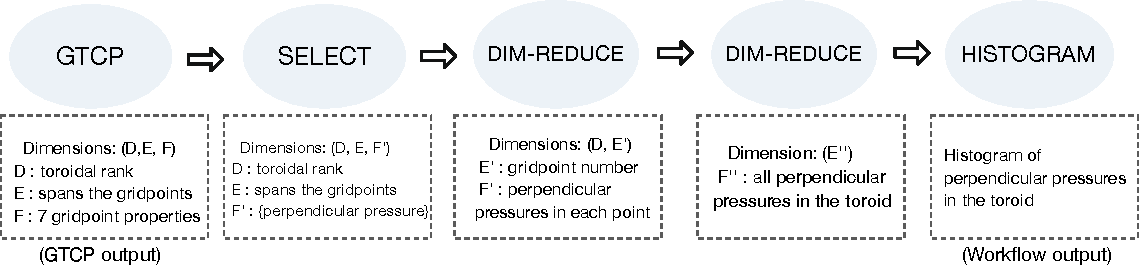
\includegraphics[width=\linewidth]{fig/wflow4}
  \vspace{-0.35in}
  \caption{GTCP Workflow}
  \label{fig:gtcp-workflow}
  \vspace{-0.15in}
\end{figure*}

\begin{figure}
  \center
  %\vspace{-0.10in}
  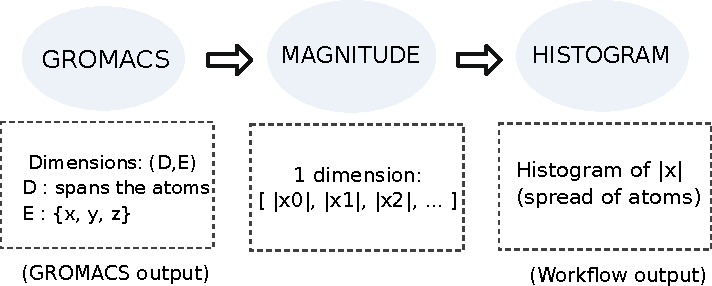
\includegraphics[width=\columnwidth]{fig/wflow_gromacs}
  \vspace{-0.25in}
  \caption{GROMACS Workflow}
  \label{fig:gromacs-workflow}
  %\vspace{-0.15in}
\end{figure}

\begin{figure}
  \begin{lstlisting}
  aprun -n 64 histogram velos.fp 16 velocities &
  aprun -n 256 magnitude lmpselect.fp lmpsel velos.fp velocities &
  aprun -n 256 select dump.custom.fp atoms 1 lmpselect.fp lmpsel vx vy vz &
  aprun -n 1024 lammps < in.cracksm &
  wait
  \end{lstlisting}
  \vspace{-0.07in}
  \caption{\sys example launch script, LAMMPS workflow}
  \label{fig:launch-script}
  %\vspace{-0.10in}
\end{figure}

We designed and implemented three realistic in situ workflows based on
scientific codes having large user bases: the LAMMPS Newtonian particle
simulator~\cite{plimpton:1997:lammps}, GTCP, a particle-in-cell Tokamak
simulator~\cite{lin:gtc}, and GROMACS,
a biomolecular dynamics code~\cite{hess2008gromacs}.
These are illustrated in
~\autoref{fig:lammps-workflow},~\autoref{fig:gtcp-workflow},
and~\autoref{fig:gromacs-workflow}.

The primary purpose of our evaluation is to demonstrate the
successful assembly and deployment of \sys workflows. In doing so, 
we also present useful
weak and strong scaling properties exhibited by \sys components
during these runs, as well as a measurement-based validation of
the componentized method to building workflows, which is inherent in the \sys approach.

The large-scale evaluation is performed on Titan, the Cray XK7 machine at Oak Ridge
National Laboratory. It consists of 18,688 nodes each with 1 16-core AMD
Opteron CPU and 32 GB of RAM. The interconnect is a Gemini network.
% There is an
% attached Nvidia Kepler K20X GPU with an additional 6 GB of memory on every
% node.

The smaller-scale results are obtained from the Falcon cluster
on the Georgia Tech campus; it is an 80-node cluster of Intel
Xeon X5660 machines, with 12 cores and 24 GB of RAM per node. 

\subsection{Workflows}

The three \sys workflows used in this evaluation perform
different kinds of runtime data analysis overall.
However, there are similarities between them.
Each driving scientific code is a simulation that
operates on a large number of units of equal size --- namely, atoms
in the case of LAMMPS and GROMACS, and grid points
in the case of GTCP (see~\autoref{fig:toroid}).
Each simulation operates over these units
with fine-grained time step granularity
and outputs the states of these units at coarse-grained
intervals. From this point on, we refer to these larger
I/O intervals as ``timesteps.''
These \textit{states} correspond to various properties
of these units, such as the positions of individual atoms or the
temperatures of individual grid points.

% Finally, addressing here the common question in reviews:
% ``why these particular components?''

All three \sys workflows based on these simulations result in a
per-timestep histogram that describes
the spread of a certain quantity of interest over these
units.  It is often the case for in situ workflows
that the resulting data set has a much smaller size than
the raw data set output by the simulation. A histogram
illustrates one such final step in a workflow
that presents a human-readable
reduction of data, and this explains our choice for
Histogram as one of the \sys components implemented for this work.

%Still, while all three workflows result in histograms,
Still, how the workflows arrive at their results varies significantly.
Histogram expects one-dimensional input data, and
our choices for Select, Dim-Reduce, and Magnitude
illustrate examples of various generic operations that tranform
different data sets into a format that the allows
one final, simple component such as Histogram to operate on.

All components of \sys workflows, including the simulation,
are launched simultaneously using a script such as
that shown in~\autoref{fig:launch-script}.
The asynchronous property of FlexPath
allows readers to block until the corresponding
writers are ready to send their data, and vice versa.
Providing the names of the input and output streams
lets the user connect any number of components
in any order.
For example, the launch script tells Magnitude
to look for an array named \texttt{lmpsel}
in a FlexPath stream named \texttt{lmpselect.fp},
which are the names used to specify the output
stream and array of Select.
Thus, this script specifies that Magnitude is
immediately downstream from Select in this workflow.
Notice, also, the decreasing numbers of processes
used in each component.

We configure LAMMPS to simulate a disruption (a ``crack'') in a thin layer of
particles and output 5 numerical properties describing each particle in the
simulation at regular timestep intervals. This corresponds to two-dimensional
data (particles as one dimension and properties of interest as another) and
among these properties are the three-dimensional components of the particles'
velocities.
Select filters out the ID and Type of the particles, keeping
the velocities. Magnitude computes the magnitudes
of these velocity vectors, outputting a one-dimension array
of these magnitudes. Histogram outputs a human-readable distribution
of the velocity magnitudes of all particles involved in this simulation.

GTCP, a code that simulates a toroidally confined plasma, splits the solid into
toroidal slices, each made up of a number of grid points. For each of these
grid points, it outputs 7 properties of the plasma such as pressure and energy
flux. This division of the toroid is illustrated in~\autoref{fig:toroid}.
The output of the simulation is therefore a three-dimensional array in which
the dimensions span: (a) toroidal ranks (toroidal slice number), (b) grid point
numbers, and (c) various properties that describe each grid point.
Of these 7 properties, Select filters out all but the pressure in each gridpoint.
However, the output of Select is still three-dimensional, and the
data must go through two instances of Dim-Reduce to allow
Histogram to operate on it, showing in the end
a distribution of the pressures in the entire toroid.

Among other quantities, GROMACS outputs
the three-dimensional coordinates
of the atoms involved in the simulation
at regular intervals.
The data array itself is two-dimensional:
3D coordinates over all atoms.
From these, we obtain a histogram of the distances
of the atoms from the origin for each timestep, showing
an evolution of the spread of the particles throughout
the simulation.

\begin{figure}
%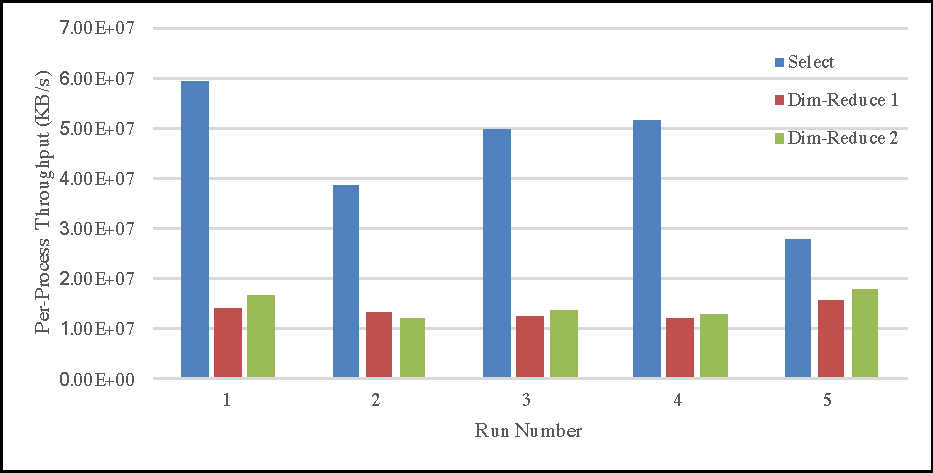
\includegraphics[width=\columnwidth]{fig/per-component-throughput}
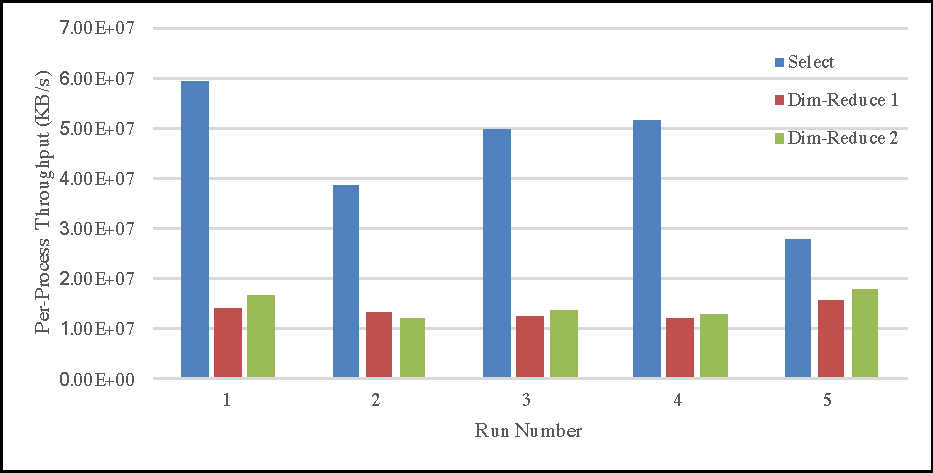
\includegraphics[width=\columnwidth]{fig/per-component-throughput}
\caption{GTCP workflow weak scaling experiment: Per-component, per-process throughputs in KB/s.}
\label{fig:gtcp-weak-perc}
\end{figure}

\subsection{Weak Scaling}
\begin{table*}[tbp]
  %\vspace{-0.15in}
  \centering
  \caption{GTCP-\sys: Weak Scaling Experiment Setup, End-to-End Results}
  \label{tab:weak-scaling-setup}
  \vspace{-0.07in}
  \begin{tabular}{|c|c|c|c|c|c|c|c|c|}
    \hline
%    SIM output & AIO time (sec) & \begin{tabular}[t]{@{}c@{}}\sys\\time (sec)\end{tabular} & LMP only (sec) \\
    Run & GTCP Output (MB) & GTCP Procs & Select Procs & Dim-Red1 Procs & Dim-Red2 Procs & Histo Procs & End2End Time (s) & Throughput (KB/s)\\
    \hline
    1 & 918.3 & 64 & 10 & 6 & 6 & 2 & 92.72 & 112,541\\
    \hline
    2 & 1434.6 & 84 & 16 & 10 & 10 & 2 & 115.23 & 102,046\\
    \hline
    3 & 2065.6 & 156 & 18 & 14 & 14 & 4 & 97.27 & 103,089\\
    \hline
    4 & 2811.3 & 234 & 25 & 19 & 19 & 5 & 96.36 & 96,605\\
    \hline
    5 & 12905.4 & 1024 & 116 & 88 & 88 & 24 & 197.66 & 48,724\\
    \hline
  \end{tabular}
  \vspace{-0.15in}
\end{table*}
Different workflows have different requirements in terms
of the data set sizes that they operate on and therefore
on the scales of their components.
Thus, in order to use \textit{generic} components, it is important
that the performance of the individual components
as well as the end-to-end performance of the resulting
workflow be reasonably predictable.
To test this, we ran a weak scaling experiment
whose setup is described in~\autoref{tab:weak-scaling-setup}.
The table lists the process sizes and data set sizes used in the 5
runs of the GTCP workflow for this experiment.
We measured the end-to-end times of these runs,
as well as the completion time of individual
timesteps, broken down by component, averaged
over the component's communicator.

These measurements allow us to extract an
approximate per-process throughput, both for
the entire workflow, end-to-end, as well as on
a per-component basis.
The last column in ~\autoref{tab:weak-scaling-setup}
lists these end-to-end results, where the total
data set size produced by the simulation is divided
by the total number of processes used in the workflow
and by the total time taken by the workflow.
~\autoref{fig:gtcp-weak-perc}
shows similar per-component, per-process throughputs for
three of the components used in these runs,
for a timestep taken arbitrarily in the workflow.
We can see that while there is a certain variation
in these throughputs across the runs, especially
at the largest scale, where communication overhead
is most significant, both \sys workflows and their
individual components exhibit very good weak scaling properties,
with a maximum throughput decrease of about 57\% between 
the two extremes in scale.

\if 0
\begin{table*}[tbp]
  %\vspace{-0.15in}
  \centering
  \caption{GTCP-\sys: Weak Scaling Experiment Results}
  \label{tab:weak-scaling-setup}
  \vspace{-0.07in}
  \begin{tabular}{|c|c|c|c|c|c|c|}
    \hline
%    SIM output & AIO time (sec) & \begin{tabular}[t]{@{}c@{}}\sys\\time (sec)\end{tabular} & LMP only (sec) \\
    Run Number & Workflow End-to-End (s) & Select Time Procs & Select Procs & Dim-Red-1 Procs & Dim-Red-2 Procs & Histo Procs\\
    \hline
    1 & 918.3 & 64 & 10 & 6 & 6 & 2\\
    \hline
    2 & 1434.6 & 84 & 16 & 10 & 10 & 2\\
    \hline
    3 & 2065.6 & 156 & 18 & 14 & 14 & 4\\
    \hline
    4 & 2811.3 & 234 & 25 & 19 & 19 & 5\\
    \hline
    5 & 12905.4 & 1024 & 116 & 88 & 88 & 24\\
    \hline
  \end{tabular}
  \vspace{-0.15in}
\end{table*}
\fi

\subsection{Comparing Generic and Ad Hoc Approaches}

\begin{table}[tbp]
  %\vspace{-0.15in}
  \centering
  \caption{LAMMPS: \sys vs. All-In-One Comparison}
  \label{tab:aio}
  \vspace{-0.07in}
  \begin{tabular}{|l|l|l|l|l|}
    \hline
    SIM output & AIO time (sec) & \begin{tabular}[t]{@{}c@{}}\sys\\time (sec)\end{tabular} & LMP only (sec) \\
    \hline
    20 MB & 115.26 & 116.51 & 115.03\\
    \hline
    80 MB & 148.70 & 149.80 & 146.97\\
    \hline
    320 MB & 154.65 & 157.65 & 153.69\\
    \hline
    1280 MB & 155.32 & 157.98 & 152.48\\
    \hline
    5120 MB & 167.39 & 168.79 & 165.22\\
    \hline
  \end{tabular}
  \vspace{-0.15in}
\end{table}

It is expected that assembling a workflow
using generic components involves the use
of finer-grain components
than when using ad-hoc analytical routines
specifically coded
for a workflow of interest.
One problem that might be anticipated
in more componentized workflows
is a decrease in overall performance caused by
(a) more stages that require the coordination
of readers and writers
and (b) more points of actual data transfer.

To investigate this potential problem,
we wrote a custom, all-in-one (AIO) component
that performs the same analytical procedure
as all the components involved in the LAMMPS workflow
outside of the simulation itself.
We measured the start-to-end completion times of the two workflows 
at different scales.

~\autoref{tab:aio} shows the start-to-end
completion times
at increasing scales, of
(a) LAMMPS with the AIO component
in the second column
(b) LAMMPS with the full \sys workflow in the 3rd column
and (c) the LAMMPS simulation only with the output routines
removed from the code in the last column.
The measurements in the last column
are meant to give an idea of the portion
of the workflow completion time taken up by the simulation
computation only.

A weak scaling approach
is used, with approximately the same
per-process data size throughout the scaling.
The time is measured from the start of the simulation
to the point when the last histogram of
the last timestep is written.
For each \sys workflow run, the corresponding
AIO workflow run allocates the same
number of processes to the AIO component
as the \sys workflow allocates to the Select component.
In the \sys workflow, additional processes
are allocated to the other two components
(Magnitude and Histogram).

The results show only a small increase in
workflow completion time for the \sys
workflows (with a maximum increase of $1.9 \%$).
The componentized
approach involves more data exchange points
in the workflow, thus leading to
overhead from increased $MxN$ coordination and data exchange.
However, the overlap of computation and I/O provided by FlexPath
amortizes this overhead.

Granted, slightly more resources are allocated to the
\sys workflow runs to allow the small number
of final components to execute (1280 processes
used in total for the AIO workflow vs. 1600 for
the \sys workflow at the largest scale).
Also, much of the start-to-end time is spent on
the simulation's computation.
However, the measurements in the last column
of \autoref{tab:aio}
only give an idea of the proportion of 
overall time occupied by the simulation only,
since when workflows are running, there is much
overlap in the computation and I/O between the
simulation and other components. All in all,
these results show that the
fine-grained component approach
to assembling workflows
is reasonable from a performance standpoint.

\subsection{Strong Scaling}
\begin{figure}
  \centering
  \vspace{-0.08in}
  \input{data/gro-mag-strong}
  \vspace{-0.12in}
  \caption{Magnitude strong scaling in the GROMACS workflow.}
  \label{fig:gtcp-strong}
  \vspace{-0.25in}
\end{figure}
To determine appropriate resources
to use in workflow runs,
we run strong scaling experiments such
as presented in~\autoref{fig:gtcp-strong},
where only one component's process size
varies.
What we generally observe is expected: a linear domain of
scalability, followed by a turning point
and eventual flattening of the scaling curve.
~\autoref{fig:gtcp-strong} shows the
linear domain of the timestep
completion time of the Magnitude component
in the GROMACS workflow; the process size of Magnitude
varies, with more processes used in the lower
end of the chart, and the process sizes of
GROMACS and Histogram are kept the same.
Such experiments allow users
to better determine how to allocate resources to \sys workflows.
While limited space only allows us to present this sample
result, numerous results we
have obtained from other components
and workflows show similar strong scaling characteristics.

\if 0
In this section we use
performance measurements on two of these workflows
to show (a) that a componentized method in
building workflows, which is inherent in the SuperGlue approach,
is valid from a performance point of view,
and (b) to show some of the scaling characteristics
of the components.
These results also serve to show that
SuperGlue workflows were successfully
deployed at various
scales.
% implicit here is that presenting
% performance measurements on the workflows
% shows more concretely that they actually *run*,
% which reinforces the statements in the
% previous section.

\if 0
The goals of the evaluation are to demonstrate the \ada{state goals
  clearly to set correct expectations, see if this is correct or needs
  to be expanded:} the feasibility of reusing
  SuperGlue components across workloads, and the ability of the
  SuperGlue components to maintain similar performance and scaling
levels as ``hand-tuned'' workflow compositions. 
\fi

The evaluation is performed on Titan, the Cray XK7 machine at Oak Ridge
National Laboratory. It consists of 18,688 nodes each with 1 16-core AMD
Opteron CPU and 32 GB of RAM. The interconnect is a Gemini network. There is an
attached Nvidia Kepler K20X GPU with an additional 6 GB of memory on every
node.

\subsection{Evaluation of Componentization}

\begin{table}[tbp]
  %\vspace{-0.15in}
  \centering
  \caption{LAMMPS SuperGlue vs. All-In-One Comparison}
  \label{tab:aio}
  \vspace{-0.07in}
  \begin{tabular}{|l|l|l|l|l|}
    \hline
    SIM output & AIO time (sec) & Superglue time (sec) & LMP only (sec) \\
    \hline
    20 MB & 115.26 & 116.51 & 115.03\\
    \hline
    80 MB & 148.70 & 149.80 & 146.97\\
    \hline
    320 MB & 154.65 & 157.65 & 153.69\\
    \hline
    1280 MB & 155.32 & 157.98 & 152.48\\
    \hline
    5120 MB & 167.39 & 168.79 & 165.22\\
    \hline
  \end{tabular}
  \vspace{-0.15in}
\end{table}

It is expected that assembling a workflow
using generic components involves the use
of finer-grain components
than when using ad-hoc analytical routines
specifically coded
for a workflow of interest.
One problem that might be anticipated
in more componentized workflows
is a decrease in overall performance caused by
(a) more stages that require the coordination
of readers and writers
and (b) more points of actual data transfer.

To investigate this potential problem,
we wrote a custom, all-in-one (AIO) component
that performs the same analytical procedure
as all the components involved in the LAMMPS workflow
(outside of the simulation itself, however).
We measured
the start-to-end completion times of the two workflows 
at different scales.

~\autoref{tab:aio} shows the start-to-end
completion times
at increasing scales, of
(a) LAMMPS with the AIO component
in the second column
(b) LAMMPS with the full SuperGlue workflow in the 3rd column
and (c) the LAMMPS simulation only with the output routines
removed from the code in the last column.
The measurements in the last column
are meant to give an idea of the portion
of the workflow completion time taken up by the simulation
computation only.

A weak scaling approach
is used, with approximately the same
per-process data size throughout the scaling.
The time is measured from the start of the simulation
to the point when the last histogram of
the last timestep is written.
For each SuperGlue workflow run, the corresponding
AIO workflow run allocates the same
number of processes to the AIO component
as the SuperGlue workflow allocates to the Select component.
In the SuperGlue workflow, additional processes
are allocated to the other two components
(Magnitude and Histogram).

The results show only a small increase in
workflow completion time for the SuperGlue
workflows (with a maximum increase of $1.9 \%$).
As mentioned previously, the componentized
approach involves more data exchange points
in the workflow, thus leading to
overhead from increased $MxN$ coordination and data exchange.
However, FlexPath allows
for asynchronous data transfer.
More specifically, when a writer writes to
a ``stream,'' it places
the data in an internal buffer
until the readers are ready to request it,
at which point a separate thread in the writer
handles the actual transfer.
This overlap
of computation and I/O
amortizes the aforementioned overhead.

Also, in the SuperGlue workflow,
the componentization of the analysis
allows for a higher level of parallelism in the overall
analysis. As an example, in the AIO component,
the Select stage of one timestep
only begins once the Magnitude
stage of the previous timestep
completes, since they exist in the same processes.
In the SuperGlue workflow, these
computational stages can run simultaneously.

Granted, more resources are allocated to the
SuperGlue workflow runs to allow the additional
components to execute.
Also, much of the start-to-end time is spent on
the simulation's computation.
However, the measurements in the last column
of \autoref{tab:aio}
only give an idea of the proportion of 
overall time occupied by the simulation only,
since when workflows are running, there is much
overlap in the computation and I/O between the
simulation and other components.
All in all, this is
an illustrative comparison that shows the validity,
from a performance angle,
of the componentized approach
to building workflows.

\subsection{Scaling}

\begin{table*}[tbp]
  \centering
  \caption{GTCP Evaluation Configuration Settings}
  \label{tab:eval-strong-gtcp}
  \vspace{-0.05in}
  \begin{tabular}{|l|l|l|l|l|l|}
    \hline
    Component Test & GTCP Procs & Select Procs & Dim-Reduce 1 & Dim-Reduce 2 & Histogram Procs \\
    \hline
    Select & 64 & $x$ & 4 & 4 & 4\\
    \hline
    Dim-Reduce 1 & 128 & 32 & $x$ & 16 & 16\\
    \hline
    Dim-Reduce 2 & 128 & 32 & 16 & $x$ & 16\\
    \hline
    %Histogram & 128 & 34 & 24 & 24 & $x$\\
    %\hline
  \end{tabular}
  \vspace{-0.07in}
\end{table*}

\begin{figure}
  \centering
  %\vspace{-0.17in}
  \input{data/gtcp-sel1-strong}
  %\vspace{-0.17in}
  \input{data/gtcp-dimr-strong}
  %\vspace{-0.06in}
  \caption{SuperGlue strong scaling in the GTCP workflow. Whole timestep
    completion time (secs) for Select and both instances of Dim-Reduce used in
    the workflow are plotted against process size}
  \label{fig:gtcp-strong}
  \vspace{-0.25in}
\end{figure}

We carried out a number of experiments
to determine some of the strong and weak scaling
characteristics of the components.

Strong scaling measurements are useful for
determining appropriate process sizes
for the components, based on the size of the
data set they operate on.
For these strong scaling measurements,
we varied the process size of a single component at
a time while fixing that of the
other components involved in the workflow,
all the while using a fixed output size from
the driving simulation.
We timed the completion of a whole timestep
taken arbitrarily in the middle of the workflow
of one component of interest at a time,
taking an average over all processes
involved in that component's timestep.

In~\autoref{fig:gtcp-strong} we show some results 
from the GTCP workflow.
The corresponding configurations (process sizes for all components)
that were used to obtain these results are listed
in~\autoref{tab:eval-strong-gtcp}.
These strong scaling results show a general trend
seen in the strong scaling experiments for SuperGlue
components: a linear domain of scalability followed
by a turning point and eventual flattening
of the curve. This shows
that given
a particular workload, users can select SuperGlue process sizes
that match their resources and performance requirements.

Similar measurements exist for the LAMMPS and GROMACS workflows.
These are available in the repository~\cite{champsaur:superglue-repo}.

The third column of~\autoref{tab:aio} already
shows promising
weak scaling characteristics of SuperGlue
in the LAMMPS workflow. That is, there is little
difference in the end-to-end
completion time of the workflow
for simulation output sizes varying
from 80 MB to 5120 MB (a factor of 64
increase in simulation output size).
For the 5120 MB run, the configuration used
was 1024 LAMMPS processes, 256 Select processes,
256 Magnitude processes, and 64 Histogram processes.

Per-component, per-timestep results
showing good weak scaling characteristics of
SuperGlue
also exist for the GTCP workflow and are also
available in~\cite{champsaur:superglue-repo}.
Space limitations prevent us
from showing them here.

\if 0
\subsection{Strong Scaling Experiments}


\begin{figure}
  \centering
  \vspace{-0.25in}
  \input{data/lmp-sel-strong}
  \vspace{-0.15in}
  \input{data/lmp-mag-strong}
  \vspace{-0.17in}
  \input{data/lmp-hist-strong}
  %  }
  %
  \vspace{-0.05in}
  \caption{SuperGlue strong scaling in the LAMMPS workflow.
    Completion time (secs) of a full timestep and of the data transfer
    portion of the same timestep are plotted against process size.}
  \label{fig:lammps-strong}
  \vspace{-0.18in}
\end{figure}

\begin{figure}
  \centering
  \vspace{-0.17in}
  \input{data/gtcp-sel1-strong}
  \vspace{-0.17in}
  \input{data/gtcp-dimr-strong}
  \vspace{-0.06in}
  \caption{SuperGlue strong scaling in the GTCP workflow. Whole timestep
    completion time (secs) for Select and both instances of Dim-Reduce used in
    the workflow are plotted against process size}
  \label{fig:gtcp-strong}
  \vspace{-0.25in}
\end{figure}

\ada{add axis labels and units to plots. }
  

\begin{table*}[tbp]
%\vspace{-0.15in}
\centering
\caption{LAMMPS Evaluation Configuration Settings}
\label{tab:eval-strong-lammps}
\vspace{-0.15in}
\begin{tabular}{|l|l|l|l|l|}
\hline
Component Test & LAMMPS Procs & Select Procs & Magnitude Procs & Histogram Procs \\
\hline
Select & 256 & $x$ & 16 & 8\\
\hline
Magnitude & 256 & 60 & $x$ & 8\\
\hline
Histogram & 256 & 32 & 16 & $x$\\
\hline
\end{tabular}
%\vspace{-0.15in}
\end{table*}

%LAMMPS setups:
%Select is 256:x:16:8
%Magnitude is 256:60:x:8
%Histogram is 256:32:16:x

\begin{table*}[tbp]
\centering
\caption{GTCP Evaluation Configuration Settings}
\label{tab:eval-strong-gtcp}
\vspace{-0.15in}
\begin{tabular}{|l|l|l|l|l|l|}
\hline
Component Test & GTCP Procs & Select Procs & Dim-Reduce 1 & Dim-Reduce 2 & Histogram Procs \\
\hline
Select & 64 & $x$ & 4 & 4 & 4\\
\hline
Dim-Reduce 1 & 128 & 32 & $x$ & 16 & 16\\
\hline
Dim-Reduce 2 & 128 & 32 & 16 & $x$ & 16\\
\hline
%Histogram & 128 & 34 & 24 & 24 & $x$\\
%\hline
\end{tabular}
\vspace{-0.07in}
\end{table*}

%GTCP setups:
%Select is 64:x:4:4:4
%Dim-Reduce1 is 128:32:x:16:16
%Dim-Reduce2 is 128:32:16:x:16
%Histogram is 128:34:24:24:x

To understand the strong scaling behavior exhibited by the components in
different scenarios, we carried out strong scaling measurements of the
components in both the LAMMPS and GTCP workflows.
To do this, we varied the process size of a single component at
a time while fixing that of the other components involved in the workflow,
and using a fixed output size from the driving simulation.  We
determined reasonable process sizes for the fixed-size components using
preliminary testing. 

The results are illustrated in~\autoref{fig:lammps-strong} and~\autoref{fig:gtcp-strong}.
Each point shows
the completion time for a single time step arbitrarily chosen in the middle of
the execution of the workflow. Depicted below the strong scaling curves
in~\autoref{fig:lammps-strong}
are the data transfer times. That is, these points
show the portion of the timestep
completion time spent by the components waiting to receive requested data.
The workflow configurations (process counts) used to obtain these measurements are shown
in~\autoref{tab:eval-strong-lammps} and~\autoref{tab:eval-strong-gtcp}.
The global output of the simulation in the LAMMPS workflow
is \SI{1.28}{\giga\byte}. In the GTCP workflow, the Select
measurements are taken using a \SI{900}{\mega\byte} output
from the simulation, and those of Dim-Reduce using a
\SI{3.8}{\giga\byte} output.
The scale used for these results is small compared to the
scale at which these simulations can be run due to
the limited time and resources available 
for the numerous complete workflows executions required
to obtain meaningful strong scaling results.

These results provide valuable information about the components.
First, they show that the components exhibit regular strong
scaling behavior. That is, 
a linear domain of scalability is followed by a turning point and an
eventual flattening out of the performance, where the benefit
of adding more processes dwindles.
That there exists a linear domain means that given
a particular workload, users can select SuperGlue process sizes
that match their resources and performance requirements.
The flat domain is long and does not show any drastic reversal
of performance. Without knowing the full strong
scaling characteristics of the SuperGlue components used in a particular workflow,
a user can safely guess a process size to use for a particular component,
using the strong scaling results from the same component with a similar
workload size, without incurring unreasonable overhead.

The turning point of scalability of a component
is not necessarily determined by
its per-process workload size.
In~\autoref{fig:lammps-strong}, the turning point of Select
occurs at a per-process workload of around \SI{32}{\mega\byte}.
Here, the global data size sent to Select
is \SI{1.28}{\giga\byte}.
In a separate set of measurements using the GTCP workflow,
the turning point of Select occurs at a per-process workload
of \SI{113}{\mega\byte}, where the global dataset size
was \SI{3.8}{\giga\byte}. Therefore, global workload size
is a factor in determining the turning point of scalability
of the SuperGlue components.

While there is communication overhead in the computation itself,~\autoref{fig:lammps-strong} shows the majority of the communication
overhead, i.e., the time spent on data transfer between components,
is small compared to the total per-timestep execution time of
the SuperGlue components. This supports the idea
of assembling workflows using numerous, simple,
generic components.

\subsection{Weak Scaling Experiments}

Additional experiments are performed for the GTCP workflow to determine the
weak scaling performance for the components. The configurations for these experiments
are presented in~\autoref{tab:eval-weak-gtcp-1}. The performance results are
presented in~\autoref{tab:eval-weak-gtcp-2}. To read the tables, match the
rows. For example, the first row in~\autoref{tab:eval-weak-gtcp-1} corresponds
to the performance results in row 1 in~\autoref{tab:eval-weak-gtcp-2}.
These runs use SuperGlue process sizes for which the per-process
workloads reside near the turning points in the
strong scaling results presented above.

Overall, the components and the overall workflow
exhibit very promising weak scaling behavior.
While there are slightly different per-process
data sizes in each row of the table for both
per-simulation process and per-SuperGlue process,
there is little variation in the timestep completion
times of the SuperGlue components and in the end-to-end
completion times of the entire workflow for different
workload sizes.

{\em Select} gets the full brunt of the total data size. Dividing the process
count into the total data size shows that on average, it is roughly the same
for weak scaling. The other components exhibit similar performance consistency.
Also note that these are not exactly identical ratios or counts.  The data size
per GTCP process is maintained as it is scaled. The amount of data each
SuperGlue component process varies a bit. Also note that there is not a fixed
n-1 ratio required for any of the components. Instead, an m-n mapping works
correctly.

%Process count ratios
%GTCP	GTCP		GTCP
%vs	vs		vs
%Select	Dim-Reduce	Histogram
%6.4	10.67		32
%5.25	8.4		41
%8.67	11.14		34
%9.36	12.31		46.8

\begin{table*}[tbp]
%\vspace{-0.15in}
\centering
\caption{GTCP Weak Scaling Evaluation Configuration Settings}
\label{tab:eval-weak-gtcp-1}
\vspace{-0.15in}
\begin{tabular}{|l|l|l|l|l|l|l|l|}
\hline
Configuration & GTCP Procs & Select Procs & Dim-Reduce 1 & Dim-Reduce 2 & Histogram Procs & Total Data Size & End-to-End Time\\
\hline
C1 & 64 & 10 & 6 & 6 & 2 & 918,303,680 & 92.724\\
\hline
C2 & 84 & 16 & 10 & 10 & 2 & 1,434,599,936 & 115.232\\
\hline
C3 & 156 & 18 & 14 & 14 & 4 & 2,065,583,520 & 97.266\\
\hline
C4 & 234 & 25 & 19 & 19 & 5 & 2,811,256,000 & 96.359\\
\hline
\end{tabular}
\vspace{-0.15in}
\end{table*}

\begin{table}[tbp]
%\vspace{-0.10in}
\centering
\caption{GTCP Weak Scaling Component Performance}
\label{tab:eval-weak-gtcp-2}
\vspace{-0.15in}
\begin{tabular}{|p{0.1 in}|p{0.67 in}|p{0.65 in}|p{0.65 in}|p{0.65 in}|}
\hline
 & Select Average Time & Dim-Reduce 1 Average Time & Dim-Reduce 2 Average Time & Histogram Average Time\\
\hline
C1 & 1.55 & 1.58 & 1.34 & 0.6\\
\hline
C2 & 2.34 & 1.58 & 1.72 & 0.78\\
\hline
C3 & 2.31 & 1.73 & 1.54 & 0.713\\
\hline
C4 & 2.19 & 1.76 & 1.68 & 0.89\\
\hline
\end{tabular}
\vspace{-0.25in}
\end{table}

\fi
\fi
